\documentclass[10pt,a4paper]{amsart}
\usepackage{amsmath,amssymb,amsthm,graphicx}
\usepackage{stmaryrd}
\usepackage{array}
\title{Fundamental theorem of substructural parametricity with purely positive recursive types}
\author{C. B. Aberlé, Karl Crary, Chris Martens, Frank Pfenning}
\date{doi:10.4230/LIPIcs.FSCD.2025.4; CC BY4.0 (official publisher HTML/PDF)}
\begin{document}
\maketitle
\noindent\textit{Editorial note.} Source https://drops.dagstuhl.de/entities/document/10.4230/LIPIcs.FSCD.2025.4. Copyright C. B. Aberlé, Karl Crary, Chris Martens and Frank Pfenning, CC BY4.0. Original statements and all printed author proof material are faithfully converted. Theorem9 is the sole counted target; base and mixed-variable fundamental theorems and illustrative consequences are supporting context. Author omissions and termination proviso are retained without supplementation.\par\medskip
\noindent\textit{Allowed standard prerequisites (editorial).}\begin{itemize}
\item Parametric logical predicates, monoids and structural induction. Publisher sections2-6 and references. The actual ordered calculus, algebraic predicate, recursive type restrictions and author proof cases are included, rather than replaced by prerequisite citations.
\end{itemize}\medskip
% BEGIN S2
 
\par\medskip\noindent\textbf{2 A Minimalist Fragment}\par
 
% BEGIN S2.p1
 
We start with a small fragment of the Lambek Calculus [25, 29], extended with parametric polymorphism [43]. This fragment is sufficient to illustrate the main ideas behind our constructions. For the sake of simplicity we choose a Curry-style formulation of typing, concentrating on properties of untyped terms rather than intrinsically typed terms. This allows the same terms to inhabit ordered, linear, and unrestricted types and thereby focus on semantic rather than syntactic issues.\par
  
\par  \quad  \[\begin{array}[]{llcll}\mbox{Types}&A,B&::=&\alpha\mid\mathbf{1}\mid A\bullet B\mid A\rightarrowtail B\mid A\twoheadrightarrow B\mid\forall\alpha.\,A\\
\mbox{Terms}&e&::=&x\\
&&\mid&()\mid\mathbf{match}\;e\;(()\Rightarrow e^{\prime})&(\mathbf{1})\\
&&\mid&(e_{1},e_{2})\mid\mathbf{match}\;e\;((x,y)\Rightarrow e^{\prime})&(A\bullet B)\\
&&\mid&\lambda x.\ e\mid e_{1}\,e_{2}&(A\rightarrowtail B,A\twoheadrightarrow B)\end{array}\]\quad  \quad  
  
In this fragment, we have $A\bullet B$ (read “$A$ fuse $B$”) which, logically, is a noncommutative conjunction. We have two forms of implication: $A\rightarrowtail B$ (read: “$A$ under $B$”, originally written as $A\mathbin{\backslash}B$) which is true if from the hypothesis $A$ placed at the left end of the antecedents we can deduce $B$, and $A\twoheadrightarrow B$ (read: “$B$ over $A$”, originally written as $B\mathbin{/}A$) which is true if from the hypothesis $A$ placed at the right end of the antecedents we can prove $B$. Lambek’s original notation was suitable for the sequent calculus and its applications in linguistics, but is less readable for natural deduction and functional programming.\par
 
% END S2.p1
 
% BEGIN S2.p2
 
Our basic typing judgment has the form $\Delta\mid\Omega\vdash e:A$ where $\Delta$ consists of hypotheses $\alpha\;\mathsf{type}$, and $\Omega$ is an ordered context $(x_{1}:A_{1})\ldots(x_{n}:A_{n})$. We make the standard presuppositions that $\Delta\vdash A\;\mathsf{type}$ and $\Delta\vdash A_{i}\;\mathsf{type}$ for every $x_{i}:A_{i}$ in $\Omega$, and that both type variables and term variables are pairwise distinct. The rules are show in Figure 1.\par
 
% END S2.p2
 
% BEGIN S2.F1

\begin{center}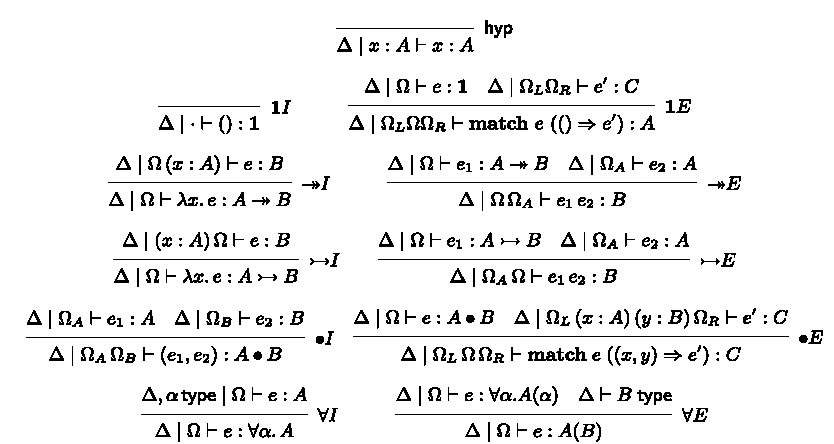
\includegraphics[width=0.95\linewidth,height=0.45\textheight,keepaspectratio]{graphic-01.pdf}\end{center}
 
Figure 1: Ordered Natural Deduction.\par
 
% END S2.F1
 
% BEGIN S2.p3
 
Here are a few example judgments that hold or fail. We elide the context $\Delta=$ $(\alpha\,\mathsf{type},\beta\,\mathsf{type},\gamma\,\mathsf{type})$.\par
  
\par  \quad  \[\begin{array}[]{lcll}&\vdash&\lambda x.\,x:\alpha\rightarrowtail\alpha\\
&\vdash&\lambda x.\,x:\alpha\twoheadrightarrow\alpha\\
&\not\vdash&\lambda x.\,\lambda y.\,x:\alpha\twoheadrightarrow(\beta\twoheadrightarrow\alpha)&(\mbox{no weakening})\\
&\not\vdash&\lambda x.\,(x,x):\alpha\twoheadrightarrow(\alpha\bullet\alpha)&(\mbox{no contraction})\\
&\vdash&\lambda x.\,\lambda y.\,(x,y):\alpha\twoheadrightarrow(\beta\twoheadrightarrow(\alpha\bullet\beta))\\
&\not\vdash&\lambda x.\,\lambda y.\,(x,y):\alpha\rightarrowtail(\beta\rightarrowtail(\alpha\bullet\beta))&(\mbox{no exchange})\\[4.30554pt]
f:\beta\twoheadrightarrow(\alpha\rightarrowtail\gamma)&\vdash&\lambda x.\,\lambda y.\,(f\,y)\,x:\alpha\rightarrowtail(\beta\twoheadrightarrow\gamma)&(\mbox{``associativity''})\\
g:\alpha\rightarrowtail(\beta\twoheadrightarrow\gamma)&\vdash&\lambda y.\,\lambda x.\,(g\,x)\,y:\beta\twoheadrightarrow(\alpha\rightarrowtail\gamma)\\[4.30554pt]
g:(\alpha\bullet\beta)\twoheadrightarrow\gamma&\vdash&\lambda x.\,\lambda y.\,g\,(x,y):\alpha\twoheadrightarrow(\beta\twoheadrightarrow\gamma)&(\mbox{currying})\\
f:\alpha\twoheadrightarrow(\beta\twoheadrightarrow\gamma)&\vdash&\lambda p.\,\mathbf{match}\;p\;((x,y)\Rightarrow f\,x\,y):(\alpha\bullet\beta)\twoheadrightarrow\gamma&(\mbox{uncurrying})\end{array}\]\quad  \quad  
  
% END S2.p3
 
% BEGIN S2.p4
 
The strictures of the typing judgment imply that certain types may be uninhabited, or may be inhabited by terms that are extensionally equivalent (i.e., that yield the same outputs for all closed inputs) to a small number of possibilities. To count the number of linear functions, translate $(A\twoheadrightarrow B)^{\mathchoice{\mathsf{L}}{\mathsf{L}}{\scriptscriptstyle\mathsf{L}}{\scriptscriptstyle\mathsf{L}}}=(A\rightarrowtail
B)^{\mathchoice{\mathsf{L}}{\mathsf{L}}{\scriptscriptstyle\mathsf{L}}{\scriptscriptstyle\mathsf{L}}}=A^{\mathchoice{\mathsf{L}}{\mathsf{L}}{\scriptscriptstyle\mathsf{L}}{\scriptscriptstyle\mathsf{L}}}\multimap B^{\mathchoice{\mathsf{L}}{\mathsf{L}}{\scriptscriptstyle\mathsf{L}}{\scriptscriptstyle\mathsf{L}}}$ and $(A\bullet B)^{\mathchoice{\mathsf{L}}{\mathsf{L}}{\scriptscriptstyle\mathsf{L}}{\scriptscriptstyle\mathsf{L}}}=A^{\mathchoice{\mathsf{L}}{\mathsf{L}}{\scriptscriptstyle\mathsf{L}}{\scriptscriptstyle\mathsf{L}}}\otimes B^{\mathchoice{\mathsf{L}}{\mathsf{L}}{\scriptscriptstyle\mathsf{L}}{\scriptscriptstyle\mathsf{L}}}$ and similarly for unrestricted functions.\par
   
\par  Types\quad  Ordered\quad  Linear\quad  Unrestricted\quad  
   
\par  $\alpha\twoheadrightarrow\alpha$\quad  1\quad  1\quad  1\quad  
 
\par  $\alpha\twoheadrightarrow(\alpha\twoheadrightarrow\alpha)$\quad  0\quad  0\quad  2\quad  
 
\par  $\alpha\twoheadrightarrow(\alpha\twoheadrightarrow(\alpha\bullet\alpha))$\quad  1\quad  2\quad  4\quad  
 
\par  $\alpha\twoheadrightarrow(\alpha\rightarrowtail(\alpha\bullet\alpha))$\quad  1\quad  2\quad  4\quad  
 
\par  $\alpha\twoheadrightarrow(\beta\twoheadrightarrow(\beta\bullet\alpha))$\quad  0\quad  1\quad  1\quad  
 
\par  $\alpha\twoheadrightarrow(\beta\twoheadrightarrow(\alpha\bullet\beta))$\quad  1\quad  1\quad  1\quad  
   
% END S2.p4
 
% BEGIN S2.p5
 
Because our intended application language based on adjoint natural deduction [19] is call-by-value, we can give a straightforward big-step operational semantics [22] relating a term to its final value. Because this evaluation does not directly interact with or benefit from substructural properties, we show it without further comment in Figure 2. It has the property of preservation that if $\cdot\vdash e:A$ and $e\mathrel{\hookrightarrow}v$ then $\cdot\vdash v:A$. Jang et al. give an account [19] that exploits linearity and other substructural properties, although not the lack of exchange.\par
 
% END S2.p5
 
% BEGIN S2.F2

\begin{center}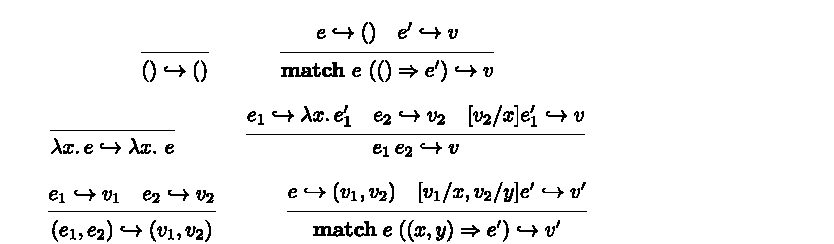
\includegraphics[width=0.95\linewidth,height=0.45\textheight,keepaspectratio]{graphic-02.pdf}\end{center}
 
Figure 2: Big-Step Operational Semantics.\par
 
% END S2.F2
 
% END S2


% BEGIN S3
 
\par\medskip\noindent\textbf{3 An Algebraic Logical Predicate}\par
 
% BEGIN S3.p1
 
Because of our particular setting, we define two mutually dependent logical predicates: $\llbracket A\rrbracket$ for closed terms and $[A]$ for closed values. In addition, the relation is parameterized by elements from an algebraic domain which may have various properties. For the ordered case, it should be a monoid, for the linear case a commutative monoid. However, the rules themselves do not require this for the pure sets of terms. We use $m\cdot n$ for the binary operation on the monoid, and $\epsilon$ for its unit.\par
 
% END S3.p1
 
% BEGIN S3.p2
 
Ignoring polymorphism for now, we write $m\Vdash e\in\llbracket A\rrbracket$ and $m\Vdash v\in[A]$, which is defined by\par
  
\par  \quad  \[\begin{array}[]{lcl}m\Vdash e\in\llbracket A\rrbracket&\Longleftrightarrow&\exists v.\,e\mathrel{\hookrightarrow}v\land m\Vdash v\in[A]\\[10.00002pt]
m\Vdash v\in[\mathbf{1}]&\Longleftrightarrow&m=\epsilon\land v=(\,)\\
m\Vdash v\in[A\bullet B]&\Longleftrightarrow&\hskip-5.0pt\begin{array}[t]{l}\exists m_{1},m_{2}.\;m=m_{1}\cdot m_{2}\land v=(v_{1},v_{2})\\
\quad\land\nobreak\ m_{1}\Vdash v_{1}\in[A]\land m_{2}\Vdash v_{2}\in[B]\end{array}\\
m\Vdash v\in[A\twoheadrightarrow B]&\Longleftrightarrow&\forall k.\,k\Vdash w\in[A]\Longrightarrow m\cdot k\Vdash v\,w\in\llbracket B\rrbracket\\
m\Vdash v\in[A\rightarrowtail B]&\Longleftrightarrow&\forall k.\,k\Vdash w\in[A]\Longrightarrow k\cdot m\Vdash v\,w\in\llbracket B\rrbracket\end{array}\]\quad  \quad  
  
We can see how the algebraic structure of the monoid tracks information about order if its operation is not commutative.\par
 
% END S3.p2
 
% BEGIN S3.p3
 
The key step, as usual in logical predicates of this nature, is the case for universal quantification and type variables. We map type variables $\alpha$ to relations $R_{B}$ between monoid elements and values in $[B]$ where $B$ is a closed type. We use $S$ to denote this mapping from type variables to sets of values and write it as a superscript on $\Vdash$.\par
  
\par  \quad  \[\begin{array}[]{lcl}m\Vdash^{S}v\in[\alpha]&\Longleftrightarrow&m\mathrel{S(\alpha)}v\\
m\Vdash^{S}v\in[\forall\alpha.\,A(\alpha)]&\Longleftrightarrow&\forall B,R_{B}.\,m\Vdash^{S,\alpha\mapsto R_{B}}v\in[A(\alpha)]\end{array}\]\quad  \quad  
  
The mapping $S$ is just passed through identically in the cases of the relation defined above.\par
 
% END S3.p3
 
% BEGIN S3.p4
 
We can already verify some interesting properties. As a first example we show that the logical predicates are nonempty.\par
 
% END S3.p4
 
% BEGIN Thmtheorem1
 
\par\medskip\noindent\textbf{Example 1.}\par
 
% BEGIN Thmtheorem1.p1
  
\par  \quad  \[\epsilon\Vdash\lambda x.\,\lambda y.\,(x,y)\in\llbracket\forall\alpha.\,\alpha\twoheadrightarrow(\alpha\twoheadrightarrow(\alpha\bullet\alpha))\rrbracket\]\quad  \quad  
  
% END Thmtheorem1.p1
 
% END Thmtheorem1
 
% BEGIN S3.SS0.SSS0.P0.SPx1
 
\par\medskip\noindent\textbf{Proof.}\par
 
% BEGIN S3.SS0.SSS0.P0.SPx1.p1
 
Because the $\lambda$-term is a value, we need to check\par
  
\par  \quad  \[\epsilon\Vdash\lambda x.\,\lambda y.\,(x,y)\in[\forall\alpha.\,\alpha\twoheadrightarrow(\alpha\twoheadrightarrow(\alpha\bullet\alpha))]\]\quad  \quad  
  
By definition, this is true if for an arbitrary $A$ and relation $m\mathrel{R_{A}}v$ we have\par
  
\par  \quad  \[\epsilon\Vdash^{\alpha\mapsto R_{A}}\lambda x.\,\lambda y.\,(x,y)\in[\alpha\twoheadrightarrow(\alpha\twoheadrightarrow(\alpha\bullet\alpha))]\]\quad  \quad  
  
Using the definition of the logical predicate for right implication twice and one intermediate step of evaluation, this holds iff\par
  
\par  \quad  \[m\cdot k\Vdash^{\alpha\mapsto R_{A}}(\lambda y.\,(v,y))\;w\in\llbracket\alpha\bullet\alpha\rrbracket\]\quad  \quad  
  
for all $m,k$ with $m\Vdash^{\alpha\mapsto R_{A}}v$ and $k\Vdash^{\alpha\mapsto R_{A}}w$. By evaluation, this is true iff\par
  
\par  \quad  \[m\cdot k\Vdash^{\alpha\mapsto R_{A}}(v,w)\in[\alpha\bullet\alpha]\]\quad  \quad  
  
Now we can apply the definition of $[A\bullet B]$, splitting $m\cdot k$ into $m$ and $k$ and reducing it to\par
  
\par  \quad  \[m\Vdash^{\alpha\mapsto R_{A}}v\in[\alpha]\land k\Vdash^{\alpha\mapsto R_{A}}w\in[\alpha]\]\quad  \quad  
  
Both of these hold because, by assumption, $m\mathrel{R_{A}}v$ and $k\mathrel{R_{A}}w$. $\hfill\blacktriangleleft$\par
 
% END S3.SS0.SSS0.P0.SPx1.p1
 
% BEGIN S3.SS0.SSS0.P0.SPx1.p2
 
More interesting, perhaps, is the reverse.\par
 
% END S3.SS0.SSS0.P0.SPx1.p2
 
% BEGIN Thmtheorem2
 
\par\medskip\noindent\textbf{Example 2.}\par
 
% BEGIN Thmtheorem2.p1
 
If\par
  
\par  \quad  \[\epsilon\Vdash e\in\llbracket\forall\alpha.\,\alpha\twoheadrightarrow(\alpha\twoheadrightarrow(\alpha\bullet\alpha))\rrbracket\]\quad  \quad  
  
then $e$ is extensionally equal to $\lambda x.\,\lambda y.\,(x,y)$, in that for any closed type $A$ and closed terms $v,w:A$, it must be the case that $e\,v\,w\hookrightarrow(v,w)$. In particular, it can not be $\lambda x.\,\lambda y.\,(y,x)$.\par
 
% END Thmtheorem2.p1
 
% END Thmtheorem2
 
% END S3.SS0.SSS0.P0.SPx1
 
% BEGIN S3.SS0.SSS0.P0.SPx2
 
\par\medskip\noindent\textbf{Proof.}\par
 
% BEGIN S3.SS0.SSS0.P0.SPx2.p1
 
We choose our monoid to be the free monoid over two generators $a$ and $b$ and we choose an arbitrary closed type $A$ and two elements $v$ and $w$. Moreoever, we pick $R_{A}$ relating only $a\mathrel{R_{A}}v$ and $b\mathrel{R_{A}}w$.\par
 
% END S3.SS0.SSS0.P0.SPx2.p1
 
% BEGIN S3.SS0.SSS0.P0.SPx2.p2
 
From the definitions (and skipping over some simple properties regarding evaluation), we obtain\par
  
\par  \quad  \[a\cdot b\Vdash^{\alpha\mapsto R_{A}}e\;v\;w\in\llbracket\alpha\bullet\alpha\rrbracket\]\quad  \quad  
  
By the clauses for $\llbracket\alpha\bullet\alpha\rrbracket$, $[\alpha\bullet\alpha]$ and $\alpha$ we conclude that\par
  
\par  \quad  \[e\;v\;w\mathrel{\hookrightarrow}(u_{1},u_{2})\]\quad  \quad  
  
for some values $u_{1}$ and $u_{2}$ with $a\mathrel{R_{A}}u_{1}$ and $b\mathrel{R_{A}}u_{2}$. Because the only value related to $a$ is $v$ and the only value related to $b$ is $w$, we conclude $u_{1}=v$ and $u_{2}=w$. Therefore\par
  
\par  \quad  \[e\;v\;w\mathrel{\hookrightarrow}(v,w)\]\quad  \quad  
  
Since $v$ and $w$ were chosen arbitrarily, we see that $e$ is extensionally equal to $\lambda x.\,\lambda y.\,(x,y)$. $\hfill\blacktriangleleft$\par
 
% END S3.SS0.SSS0.P0.SPx2.p2
 
% END S3.SS0.SSS0.P0.SPx2
 
% END S3


% BEGIN S4
 
\par\medskip\noindent\textbf{4 The Fundamental Theorem}\par
 
% BEGIN S4.p1
 
The fundamental theorem of logical predicates states that every well-typed term is in the predicate. Our relations also include terms that are not well-typed, which can occasionally be useful when one exceeds the limits of static typing.\par
 
% END S4.p1
 
% BEGIN S4.p2
 
We need a few standard lemmas, adapted to this case. We only spell out one.\par
 
% END S4.p2
 
% BEGIN Thmtheorem3
 
\par\medskip\noindent\textbf{Lemma 3 (Compositionality).}\par
 
% BEGIN Thmtheorem3.p1
 
Define $R_{A}$ such that $k\mathrel{R_{A}}w$ iff $k\Vdash w\in[A]$. Then $m\Vdash^{S,\alpha\mapsto R_{A}}v\in[B(\alpha)]$ iff $m\Vdash^{S}v\in[B(A)]$\par
 
% END Thmtheorem3.p1
 
% END Thmtheorem3
 
% BEGIN S4.SS0.SSS0.P0.SPx1
 
\par\medskip\noindent\textbf{Proof.}\par
 
% BEGIN S4.SS0.SSS0.P0.SPx1.p1
 
By induction on $B(\alpha)$. $\hfill\blacktriangleleft$\par
 
% END S4.SS0.SSS0.P0.SPx1.p1
 
% BEGIN S4.SS0.SSS0.P0.SPx1.p2
 
We would like to prove the fundamental theorem by induction over the structure of the typing derivation. Since our logical relation is defined for closed terms, we need a closing substitution $\eta$, i.e., a substitution of closed terms into the typing context of the term $e$ for which we seek to prove the fundamental theorem by induction, such that the application $\eta(e)$ of $\eta$ to $e$ is a closed term. We therefore extend the definition of the logical relation to substitutions and contexts as follows:\par
 
% END S4.SS0.SSS0.P0.SPx1.p2
 
% BEGIN S4.SS0.SSS0.P0.SPx1.p3
  
\par  \quad  \[\begin{array}[]{lcl}m\Vdash^{S}(x\mapsto v)\in[x:A]&\Longleftrightarrow&m\Vdash^{S}v\in[A]\\
m\Vdash^{S}(\eta_{1}\,\eta_{2})\in[\Omega_{1}\,\Omega_{2}]&\Longleftrightarrow&\exists m_{1},m_{2}.\,m=m_{1}\cdot m_{2}\land m_{1}\Vdash^{S}\eta_{1}\in[\Omega_{1}]\land m_{2}\Vdash^{S}\eta_{2}\in[\Omega_{2}]\\
m\Vdash^{S}(\cdot)\in[\cdot]&\Longleftrightarrow&m=\epsilon\end{array}\]\quad  \quad  
  
Due to the associativity of the monoid operation and concatenation of contexts, this constitutes a valid definition.\par
 
% END S4.SS0.SSS0.P0.SPx1.p3
 
% BEGIN Thmtheorem4
 
\par\medskip\noindent\textbf{Theorem 4 (Fundamental Theorem (purely ordered)).}\par
 
% BEGIN Thmtheorem4.p1
 
Assume $\Delta\mid\Omega\vdash e:A$, a mapping $S$ with domain $\Delta$, and closing substitution $m\Vdash^{S}\eta\in[\Omega]$. Then $m\Vdash^{S}\eta(e)\in\llbracket A\rrbracket$.\par
 
% END Thmtheorem4.p1
 
% END Thmtheorem4
 
% END S4.SS0.SSS0.P0.SPx1
 

% BEGIN S4.SS0.SSS0.P0.SPx2
 
\par\medskip\noindent\textbf{Proof.}\par
 
% BEGIN S4.SS0.SSS0.P0.SPx2.p1
 
By induction on the structure of the given typing derivation. We show a few cases.\par
  Case:  
% BEGIN S4.I1.ix1.p1
 
\begin{center}
\includegraphics[width=0.95\linewidth,height=0.45\textheight,keepaspectratio]{graphic-03.pdf}\end{center}
 
% END S4.I1.ix1.p1
 
% BEGIN S4.I1.ix1.p2
 
Then $m\Vdash^{S}\eta(x)\in[A]$ by assumption and definition, and $m\Vdash^{S}\eta(x)\in\llbracket A\rrbracket$ since $\eta(x)$ is a value.\par
 
% END S4.I1.ix1.p2
  Case:  
% BEGIN S4.I1.ix2.p1
 
\begin{center}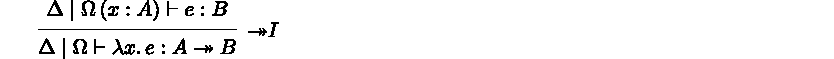
\includegraphics[width=0.95\linewidth,height=0.45\textheight,keepaspectratio]{graphic-04.pdf}\end{center}
 
% END S4.I1.ix2.p1
 
% BEGIN S4.I1.ix2.p2
  
\par   $m\Vdash^{S}\eta\in[\Omega]$ Given\quad  
 
\par   $k\Vdash^{S}v\in[A]$ Assumption (1)\quad  
 
\par   $k\Vdash^{S}(x\mapsto v)\in[x:A]$ By definition\quad  
 
\par   $m\cdot k\Vdash^{S}(\eta,x\mapsto v)\in[\Omega\,(x:A)]$ By definition\quad  
 
\par   $m\cdot k\Vdash^{S}(\eta,x\mapsto v)(e)\in\llbracket B\rrbracket$ By ind. hyp.\quad  
 
\par   $m\cdot k\Vdash^{S}(\eta(\lambda x.\,e))\,v\in\llbracket B\rrbracket$ By reverse evaluation, $v$ closed\quad  
 
\par   $m\Vdash^{S}\eta(\lambda x.\,e)\in[A\twoheadrightarrow B]$ By definition, discharging (1)\quad  
 
\par   $m\Vdash^{S}\eta(\lambda x.\,e)\in\llbracket A\twoheadrightarrow B\rrbracket$ By definition\quad  
  
% END S4.I1.ix2.p2
  Case:  
% BEGIN S4.I1.ix3.p1
 
\begin{center}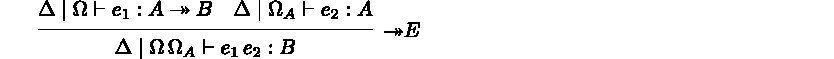
\includegraphics[width=0.95\linewidth,height=0.45\textheight,keepaspectratio]{graphic-05.pdf}\end{center}
 
% END S4.I1.ix3.p1
 
% BEGIN S4.I1.ix3.p2
  
\par   $m\Vdash^{S}\eta\in[\Omega\,\Omega_{A}]$ Given\quad  
 
\par   $m_{1}\Vdash^{S}\eta_{1}\in[\Omega]$ and $m_{2}\Vdash^{S}\eta_{2}\in[\Omega_{A}]$\quad  
 
\par  for some $m_{1}$, $m_{2}$, $\eta_{1}$, and $\eta_{2}$ with $m=m_{1}\cdot m_{2}$ and $\eta=\eta_{1}\;\eta_{2}$ By definition\quad  
 
\par   $m_{1}\Vdash^{S}\eta_{1}(e_{1})\in\llbracket A\twoheadrightarrow B\rrbracket$ By ind. hyp.\quad  
 
\par   $m_{2}\Vdash^{S}\eta_{2}(e_{2})\in\llbracket A\rrbracket$ By ind. hyp.\quad  
 
\par   $\eta_{1}(e_{1})\mathrel{\hookrightarrow}v_{1}$ with $m_{1}\Vdash^{S}v_{1}\in[A\twoheadrightarrow B]$ By definition\quad  
 
\par   $\eta_{2}(e_{2})\mathrel{\hookrightarrow}v_{2}$ with $m_{2}\Vdash^{S}v_{2}\in[A]$ By definition\quad  
 
\par   $m_{1}\cdot m_{2}\Vdash^{S}v_{1}\,v_{2}\in\llbracket B\rrbracket$ By definition\quad  
 
\par   $(\eta_{1}\,\eta_{2})(e_{1}\,e_{2})=(\eta_{1}(e_{1}))\,(\eta_{2}(e_{2}))$ By properties of substitution\quad  
 
\par   $m\Vdash^{S}\eta(e_{1}\,e_{2})\in\llbracket B\rrbracket$ Since $m=m_{1}\cdot m_{2}$ and $\eta=(\eta_{1}\,\eta_{2})$\quad  
  
% END S4.I1.ix3.p2
  Case:  
% BEGIN S4.I1.ix4.p1
 
\begin{center}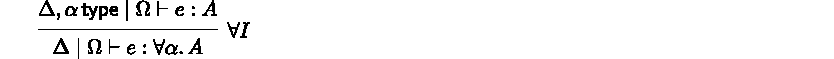
\includegraphics[width=0.95\linewidth,height=0.45\textheight,keepaspectratio]{graphic-06.pdf}\end{center}
 
% END S4.I1.ix4.p1
 
% BEGIN S4.I1.ix4.p2
  
\par   $m\Vdash^{S}\eta\in[\Omega]$ Given\quad  
 
\par   $R_{B}$ an arbitrary relation $k\mathrel{R_{B}}v$ Assumption (1)\quad  
 
\par   $m\Vdash^{S,\alpha\mapsto R_{B}}\eta\in[\Omega]$ Since $\alpha$ fresh\quad  
 
\par   $m\Vdash^{S,\alpha\mapsto R_{B}}\eta(e)\in\llbracket A\rrbracket$ By ind. hyp.\quad  
 
\par   $m\Vdash^{S}\eta(e)\in\llbracket\forall\alpha.\,A\rrbracket$ By definition, discharging (1)\quad  
  
% END S4.I1.ix4.p2
  Case:  
% BEGIN S4.I1.ix5.p1
 
\begin{center}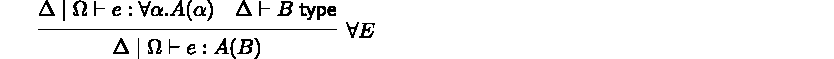
\includegraphics[width=0.95\linewidth,height=0.45\textheight,keepaspectratio]{graphic-07.pdf}\end{center}
 
% END S4.I1.ix5.p1
 
% BEGIN S4.I1.ix5.p2
  
\par   $m\Vdash^{S}\eta\in[\Omega]$ Given\quad  
 
\par   $m\Vdash^{S}\eta(e)\in\llbracket\forall\alpha.\,A(\alpha)\rrbracket$ By ind. hyp.\quad  
 
\par  Define $k\mathrel{R}_{B}v$ iff $k\Vdash^{S}v\in[B]$\quad  
 
\par   $m\Vdash^{S,\alpha\mapsto R_{B}}\eta(e)\in\llbracket A(\alpha)\rrbracket$ By definition\quad  
 
\par   $m\Vdash^{S,\alpha\mapsto R_{B}}v\in[A(\alpha)]$ for $\eta(e)\mathrel{\hookrightarrow}v$ By definition\quad  
 
\par   $m\Vdash^{S}v\in[A(B)]$ By compositionality (Lemma 3)\quad  
 
\par   $m\Vdash^{S}\eta(e)\in\llbracket A(B)\rrbracket$ By definition\quad  
  
% END S4.I1.ix5.p2
   
$\hfill\blacktriangleleft$\par
 
% END S4.SS0.SSS0.P0.SPx2.p1

% BEGIN S4.SS0.SSS0.P0.SPx2.p2
 
Because typing implies that the logical predicate holds, the earlier examples now apply to well-typed terms.\par
 
% END S4.SS0.SSS0.P0.SPx2.p2
 
% BEGIN Thmtheorem5
 
\par\medskip\noindent\textbf{Theorem 5 (Example 2 revisited).}\par
 
% BEGIN Thmtheorem5.p1
 
If\par
  
\par  \quad  \[\cdot\vdash e:\forall\alpha.\,\alpha\twoheadrightarrow(\alpha\twoheadrightarrow(\alpha\bullet\alpha))\]\quad  \quad  
  
then $e$ is extensionally equivalent to $\lambda x.\,\lambda y.\,(x,y)$.\par
 
% END Thmtheorem5.p1
 
% END Thmtheorem5
 
% END S4.SS0.SSS0.P0.SPx2
 
% BEGIN S4.SS0.SSS0.P0.SPx3
 
\par\medskip\noindent\textbf{Proof.}\par
 
% BEGIN S4.SS0.SSS0.P0.SPx3.p1
 
We just note that\par
  
\par  \quad  \[\epsilon\Vdash e\in\llbracket\forall\alpha.\,\alpha\twoheadrightarrow(\alpha\twoheadrightarrow(\alpha\bullet\alpha))\rrbracket\]\quad  \quad  
  
since $(\cdot)\in[\cdot]$ and $(\cdot)e=e$ and the empty mapping $S$ suffices without any free type variables. Then we appeal to the reasoning in Example 2. $\hfill\blacktriangleleft$\par
 
% END S4.SS0.SSS0.P0.SPx3.p1
 
% END S4.SS0.SSS0.P0.SPx3
 
% END S4


% BEGIN S5
 
\par\medskip\noindent\textbf{5 Unrestricted Functions}\par
 
% BEGIN S5.p1
 
We are interested in properties of functions such as list append or list reversal, or higher-order functions such as fold. This requires inductive types, but the functions on them are not used linearly. For example, append has a recursive call in the case of a nonempty list, but none in the case of an empty list. We could introduce a general modality ${!}A$ for this purpose. A simpler alternative that is sufficient for our situation is to introduce unrestricted function types $A\mathbin{\rightarrow}B$ (usually coded as ${!}A\multimap B$ in linear logic or ${!}A\twoheadrightarrow B$ in ordered logic). This path has been explored previously [37] with different motivations. There, an open logical relation was defined on the negative monomorphic fragment in order to show the existence of canonical forms, a property that is largely independent of ordered typing.\par
 
% END S5.p1
 
% BEGIN S5.p2
 
Adding unrestricted functions is rather straightforward in typing by using two kinds of variables: those that are ordered and those unrestricted. Then, in the logical predicate, unrestricted variables must not use any resources, that is, they are assigned the unit element $\epsilon$ of the monoid during the definition.\par
 
% END S5.p2
 
% BEGIN S5.p3
 
The generalized judgment has the form $\Delta\mid\Gamma\mathrel{;}\Omega\vdash e:A$ where $\Gamma$ contains type assignments for variables that can be used in an unrestricted (not linear and not ordered) way. All the previous rules are augmented by propagating $\Gamma$ from the conclusion to all premises. Because our term language is untyped, no extensions are needed there. Similarly, the rules of our dynamics do not need to change.\par
 
% END S5.p3
 
% BEGIN S5.F3

\begin{center}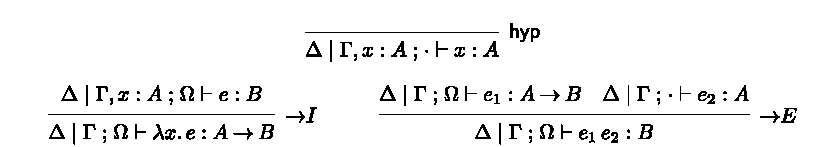
\includegraphics[width=0.95\linewidth,height=0.45\textheight,keepaspectratio]{graphic-08.pdf}\end{center}
 
Figure 3: Unrestricted functions.\par
 
% END S5.F3
 
% BEGIN S5.p4
 
We extend the logical predicate using arguments not afforded any resources.\par
 
% END S5.p4
 
% BEGIN S5.p5
 
\begin{center}
\includegraphics[width=0.95\linewidth,height=0.45\textheight,keepaspectratio]{graphic-09.pdf}\end{center}
 
% END S5.p5
 
% BEGIN S5.p6
 
The fundamental theorem extends in a straightforward way.\par
 
% END S5.p6
 
% BEGIN Thmtheorem6
 
\par\medskip\noindent\textbf{Theorem 6 (Fundamental Theorem (mixed ordered/unrestricted)).}\par
 
% BEGIN Thmtheorem6.p1
 
Assume $\Delta\mid\Gamma\mathrel{;}\Omega\vdash e:A$, a mapping $S$ with domain $\Delta$, and two closing substitutions $\epsilon\Vdash^{S}\theta\in[\Gamma]$ and $m\Vdash^{S}\eta\in[\Omega]$. Then $m\Vdash^{S}(\theta\mathrel{;}\eta)(e)\in\llbracket A\rrbracket$.\par
 
% END Thmtheorem6.p1
 
% END Thmtheorem6
 

% BEGIN S5.SS0.SSS0.P0.SPx1
 
\par\medskip\noindent\textbf{Proof.}\par
 
% BEGIN S5.SS0.SSS0.P0.SPx1.p1
 
By induction on the structure of the given typing derivation. $\hfill\blacktriangleleft$\par
 
% END S5.SS0.SSS0.P0.SPx1.p1

% BEGIN S5.SS0.SSS0.P0.SPx1.p2
 
An interesting side effect of these definitions is that if we omit ordered functions but retain pairs we obtain the “usual” formulation of closed logical predicates, including certain consequences of parametricity for the ordinary $\lambda$-calculus.\par
 
% END S5.SS0.SSS0.P0.SPx1.p2
 
% BEGIN Thmtheorem7
 
\par\medskip\noindent\textbf{Theorem 7.}\par
 
% BEGIN Thmtheorem7.p1
 
If\par
  
\par  \quad  \[\cdot\vdash e:\forall\alpha.\,\alpha\mathbin{\rightarrow}(\alpha\mathbin{\rightarrow}(\alpha\bullet\alpha))\]\quad  \quad  
  
then $e$ is extensionally equivalent to one of 4 functions: $\lambda x.\,\lambda y.\,(x,y)$, $\lambda x.\,\lambda y.\,(y,x)$, $\lambda x.\,\lambda y.\,(x,x)$, or $\lambda x.\,\lambda y.\,(y,y)$.\par
 
% END Thmtheorem7.p1
 
% END Thmtheorem7
 
% END S5.SS0.SSS0.P0.SPx1
 
% BEGIN S5.SS0.SSS0.P0.SPx2
 
\par\medskip\noindent\textbf{Proof.}\par
 
% BEGIN S5.SS0.SSS0.P0.SPx2.p1
 
By the fundamental theorem, we have\par
  
\par  \quad  \[\epsilon\Vdash e\in\llbracket\forall\alpha.\,\alpha\mathbin{\rightarrow}(\alpha\mathbin{\rightarrow}(\alpha\bullet\alpha))\rrbracket\]\quad  \quad  
  
We use this for an abitrary closed type $A$ with two arbitary values $v$, and $w$ and relation $R_{A}$ with $\epsilon\mathrel{R_{A}}v$ and $\epsilon\mathrel{R_{A}}w$. Exploiting the definition, we get\par
  
\par  \quad  \[\epsilon\Vdash^{\alpha\mapsto R_{A}}e\in\llbracket\alpha\mathbin{\rightarrow}(\alpha\mathbin{\rightarrow}(\alpha\bullet\alpha))\rrbracket\]\quad  \quad  
  
Using the definition of function twice and skipping over some evaluation and reverse evaluation, we obtain\par
  
\par  \quad  \[\epsilon\Vdash^{\alpha\mapsto R_{A}}e\,v\,w\in\llbracket\alpha\bullet\alpha\rrbracket\]\quad  \quad  
  
This means that $e\,v\,w\mathrel{\hookrightarrow}(u_{1},u_{2})$ with $\epsilon\mathrel{R_{A}}u_{1}$ and $\epsilon\mathrel{R_{A}}u_{2}$. Because of the definition of $R_{A}$ there are 4 possibilities for $(u_{1},u_{2})$, namely $(v,w)$, $(w,v)$, $(v,v)$ and $(w,w)$. This in turn means $e$ is extensionally equal to one of the 4 functions shown. $\hfill\blacktriangleleft$\par
 
% END S5.SS0.SSS0.P0.SPx2.p1
 
% END S5.SS0.SSS0.P0.SPx2
 
% END S5


% BEGIN S6
 
\par\medskip\noindent\textbf{6 Sums, Twist, and Recursive Types}\par
 
% BEGIN S6.p1
 
At this point, we are at a crossroads. Because we would like to prove theorems regarding more complex data structures such as lists, trees, or streams, we could extend the development with general inductive and coinductive types and their recursors. We conjecture that this is possible and leave it to future work. The other path is to work with purely positive types, including recursive ones whose values can be directly observed. In this approach, the definition of the logical predicate is quite easy to extend. It becomes a nested inductive definition: either the type becomes smaller or, once we encounter a purely positive type and recursion is possible, from then on the terms become strictly smaller. In this paper we take the latter approach, which excludes coinductive types such as streams from consideration, but still yields many interesting and intuitive consequences.\par
 
% END S6.p1
 
% BEGIN S6.p2
 
We take the opportunity to also round out our language with sums and twist (the symmetric counterpart of fuse). We use a signature defining equirecursive type names that may be arbitrarily mutually recursive. Because such type definitions are otherwise closed, they constitute metavariables in the sense of contextual modal type theory [31]. Each type definition $F[\Delta]=A^{+}$ (for $\Delta$ a context of type variables as in previous sections) must be contractive, that is, its definiens cannot be be another type name. Moreover, $A^{+}$ must be purely positive, which is interpreted inductively.\par
  
\par  \quad  \[\begin{array}[]{llcll}\mbox{Types}&A&::=&\ldots\mid A\mathbin{\circ}B\mid\oplus\{\ell:A_{\ell}\}_{\ell\in L}\\
\mbox{Purely Positive Types}&A^{+},B^{+}&::=&A^{+}\bullet B^{+}\mid A^{+}\mathbin{\circ}B^{+}\mid\mathbf{1}\mid\oplus\{\ell:A_{\ell}^{+}\}_{\ell\in L}\mid F[\theta]\\
\mbox{Type Definitions}&\Sigma&::=&F[\Delta]=A^{+}\mid(\cdot)\mid\Sigma_{1},\Sigma_{2}\\
\mbox{Type Substitutions}&\theta&::=&\alpha\mapsto A^{+}\mid(\cdot)\mid\theta_{1}\,\theta_{2}\\[10.00002pt]
\end{array}\]\quad  \quad  
  
The language of terms does not change much because type names are equirecursive.\par
  
\par  \quad  \[\begin{array}[]{llcll}\mbox{Term}&e&::=&\ldots\\
&&\mid&k(e)\mid\mathbf{match}\;e\;\{\ell(x_{\ell})\Rightarrow e^{\prime}\}_{\ell\in L}&(\oplus\{\ell:A_{\ell}\})\end{array}\]\quad  \quad  
  
We add the type $A\mathbin{\circ}B$ (“twist”), symmetric to $A\bullet B$, since encoding it as $B\bullet A$ requires rewriting terms, flipping the order of pairs. For $A\mathbin{\circ}B$ it is merely the typechecking that changes. This allows more types to be assigned to the same term. We allow silent unfolding of type definitions, so there are no explicit rules for $F[\theta]$.\par
 
% END S6.p2
 
% BEGIN S6.F4

\begin{center}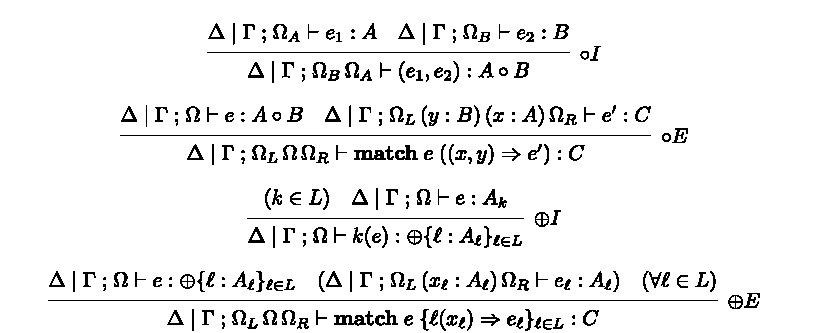
\includegraphics[width=0.95\linewidth,height=0.45\textheight,keepaspectratio]{graphic-10.pdf}\end{center}
 
Figure 4: Ordered Natural Deduction, Extended.\par
 
% END S6.F4
 
% BEGIN S6.F5

\begin{center}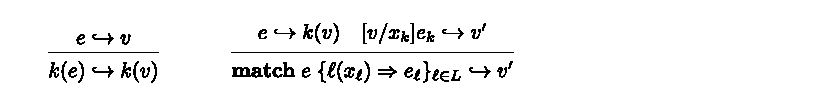
\includegraphics[width=0.95\linewidth,height=0.45\textheight,keepaspectratio]{graphic-11.pdf}\end{center}
 
Figure 5: Big-Step Operational Semantics, Extended.\par
 
% END S6.F5
 
% BEGIN S6.p3
 
The logical predicate is also extended in a straightforward manner. We assume the signature $\Sigma$ is fixed and therefore do not carry it explicitly through the definitions.\par
  
\par  \quad  \[\begin{array}[]{lcl}m\Vdash^{S}v\in[A\mathbin{\circ}B]&\Longleftrightarrow&\exists m_{1},m_{2}.\;m=m_{2}\cdot m_{1}\land v=(v_{1},v_{2})\\
&&\hbox{}\land m_{1}\Vdash^{S}v_{1}\in[A]\land m_{2}\Vdash^{S}v_{2}\in[B]\\
m\Vdash^{S}k(v)\in[{\oplus}\{\ell:A_{\ell}\}_{\ell\in L}]&\Longleftrightarrow&m\Vdash^{S}v\in[A_{k}]\land k\in L\\
m\Vdash^{S}v\in[F[\theta]]&\Longleftrightarrow&m\Vdash^{S}v\in\theta(A^{+})\ \mbox{where $F[\Delta]=A^{+}\in\Sigma$}\end{array}\]\quad  \quad  
  
% END S6.p3
 
% BEGIN S6.p4
 
Because we have equirecursive type definitions, the last clause is usually applied silently. The definition of the logical predicate is no longer straightforwardly inductive on the structure of the type. However, we see that for purely positive types (the only ones involved in recursion), the value in the definition becomes strictly smaller in each clause if type definitions are contractive. In other words, we now have a nested inductive definition of the logical predicate, first on the type, and when the type is purely positive, on the structure of the value.\par
 
% END S6.p4
 
% BEGIN S6.p5
 
We can also add recursion to our term language with the key proviso that we either restrict ourselves to certain patterns of recursion (for example, primitive recursion), or termination is guaranteed by other external means (for example, an analysis using sized types [2]). This assumption allows us to maintain the structure of the logical predicate, even if it is no longer a means to prove termination (which we are not interested in for this paper).\par
 
% END S6.p5
 
% BEGIN Thmtheorem8
 
\par\medskip\noindent\textbf{Lemma 8 (Compositionality (including purely positive equirecursive types)).}\par
 
% BEGIN Thmtheorem8.p1
 
Define $R_{A}$ such that $k\mathrel{R_{A}}w$ iff $k\Vdash w\in[A]$. Then $m\Vdash^{S,\alpha\mapsto R_{A}}v\in[B(\alpha)]$ iff $m\Vdash^{S}v\in[B(A)]$.\par
 
% END Thmtheorem8.p1
 
% END Thmtheorem8
 

% BEGIN S6.SS0.SSS0.P0.SPx1
 
\par\medskip\noindent\textbf{Proof.}\par
 
% BEGIN S6.SS0.SSS0.P0.SPx1.p1
 
By nested induction on the definition of the logical predicate for $B(\alpha)$, first on the structure of $B$ and second on the structure of the value when a purely positive type $F[\theta]$ has been reached. $\hfill\blacktriangleleft$\par
 
% END S6.SS0.SSS0.P0.SPx1.p1

% BEGIN Thmtheorem9
 
\par\medskip\noindent\textbf{Theorem 9 (Fundamental Theorem (including purely positive recursive types)).}\par
 
% BEGIN Thmtheorem9.p1
 
Assume $\Delta\mid\Gamma\mathrel{;}\Omega\vdash e:A$, a mapping $S$ with domain $\Delta$, and two closing substitutions $\epsilon\Vdash^{S}\theta\in[\Gamma]$ and $m\Vdash^{S}\eta\in[\Omega]$. Then $m\Vdash^{S}(\theta\mathrel{;}\eta)(e)\in\llbracket A\rrbracket$.\par
 
% END Thmtheorem9.p1
 
% END Thmtheorem9

% BEGIN S6.SS0.SSS0.P0.SPx2
 
\par\medskip\noindent\textbf{Proof.}\par
 
% BEGIN S6.SS0.SSS0.P0.SPx2.p1
 
By induction on the structure of the given typing derivation. When reasoning about functions and recursion, we need the assumption of termination. $\hfill\blacktriangleleft$\par
 
% END S6.SS0.SSS0.P0.SPx2.p1
 
% END S6.SS0.SSS0.P0.SPx2

% BEGIN A1
 
\par\medskip\noindent\textbf{Appendix A Complete definition of the Type System}\par
 
% BEGIN A1.p1
  
\par  \quad  \[\begin{array}[]{llcll}\mbox{Types}&A,B&::=&\alpha\mid 1\mid A\bullet B\mid A\rightarrowtail B\mid A\twoheadrightarrow B\mid\forall\alpha.\,A\\
&&\mid&A\to B\mid A\circ B\mid\oplus\{\ell:A_{\ell}\}_{\ell\in L}\end{array}\]\quad  \quad  
   
\par  \quad  \[\begin{array}[]{llcl}\mbox{Purely Positive Types}&A^{+},B^{+}&::=&A^{+}\bullet
B^{+}\mid A^{+}\circ B^{+}\\
&&\mid&\mathbf{1}\mid\oplus\{\ell:A^{+}_{\ell}\}_{\ell\in L}\mid F[\theta]\end{array}\]\quad  \quad  
   
\par  \quad  \[\begin{array}[]{llcl}\mbox{Type Definitions}&\Sigma&::=&F[\Delta]=A^{+}\mid(\cdot)\mid\Sigma_{1},\Sigma_{2}\end{array}\]\quad  \quad  
   
\par  \quad  \[\begin{array}[]{llcl}\mbox{Type Substitutions}&\theta&::=&\alpha\mapsto A^{+}\mid(\cdot)\mid\theta_{1}\theta_{2}\end{array}\]\quad  \quad  
   
\par  \quad  \[\begin{array}[]{llcll}\mbox{Terms}&e&::=&x\\
&&\mid&()\mid\mathbf{match}\;e\;(()\Rightarrow e^{\prime})&(\mathbf{1})\\
&&\mid&(e_{1},e_{2})\mid\mathbf{match}\;e\;((x,y)\Rightarrow e^{\prime})&(A\bullet B)\\
&&\mid&\lambda x.\ e\mid e_{1}\,e_{2}&(A\rightarrowtail B,A\twoheadrightarrow B,A\to B)\\
&&\mid&k(e)\mid\mathbf{match}\nobreak\ e\nobreak\ \{\ell(x_{\ell})\Rightarrow e^{\prime}\}_{\ell\in L}&(\oplus\{\ell:A_{\ell}\})\end{array}\]\quad  \quad  
  
% END A1.p1
 
% BEGIN A1.p2
 
Typing rules:\par
 
% END A1.p2
 
% BEGIN A1.p3
 
\begin{center}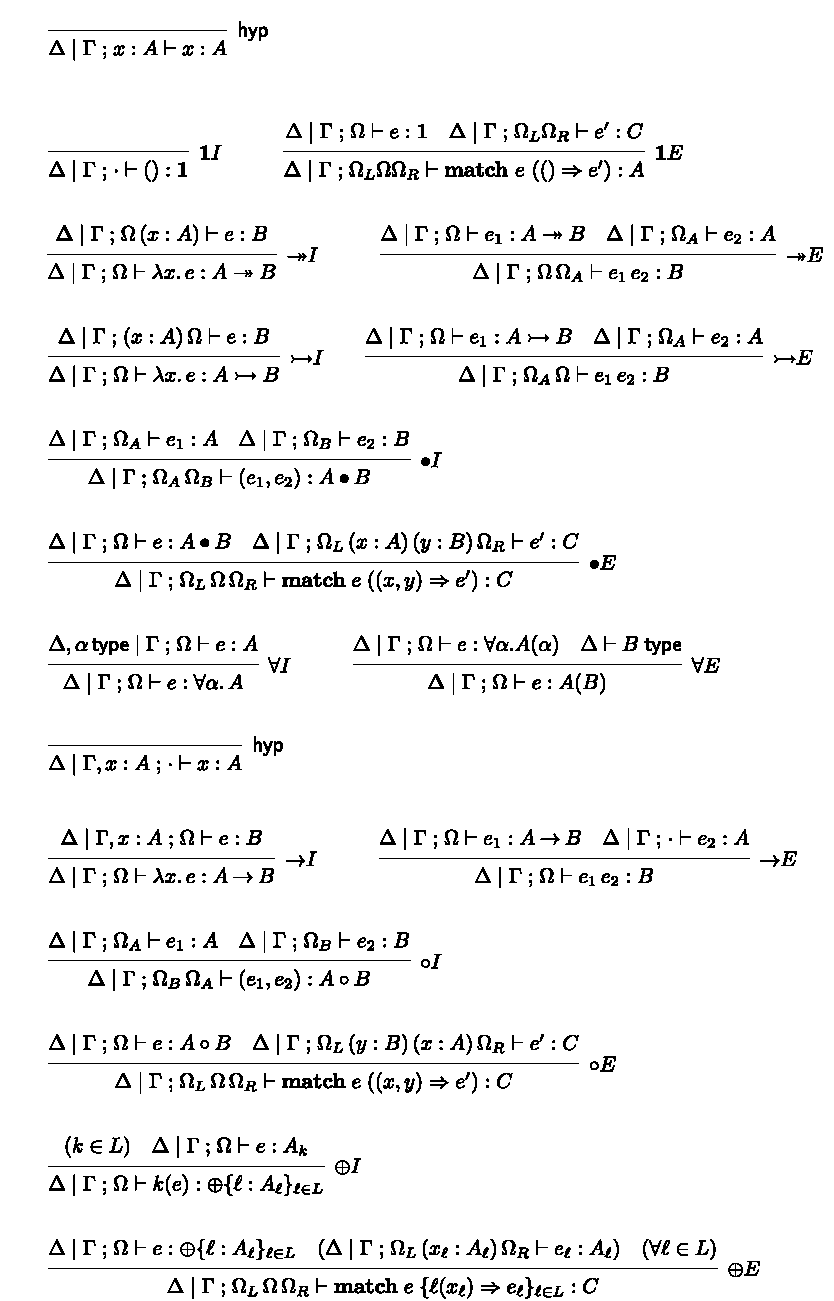
\includegraphics[width=0.95\linewidth,height=0.45\textheight,keepaspectratio]{graphic-13.pdf}\end{center}
 
% END A1.p3
 
% BEGIN A1.p4
 
Operational semantics:\par
 
% END A1.p4
 
% BEGIN A1.p5
 
\begin{center}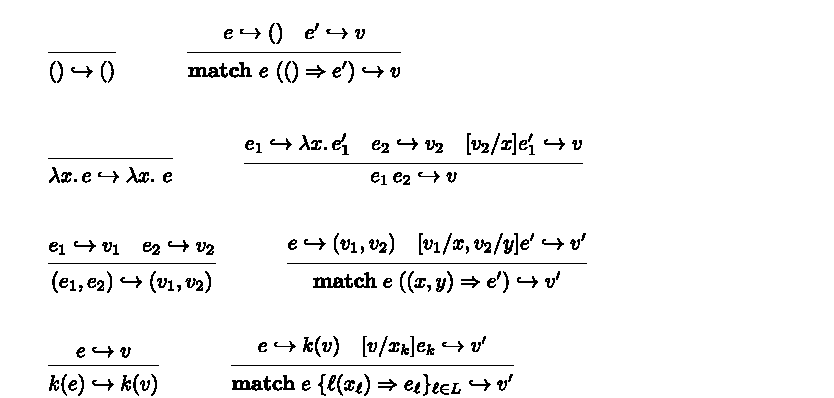
\includegraphics[width=0.95\linewidth,height=0.45\textheight,keepaspectratio]{graphic-14.pdf}\end{center}
 
% END A1.p5
 
% END A1


% BEGIN A2
 
\par\medskip\noindent\textbf{Appendix B Complete definition of the Logical Predicate}\par
 
% BEGIN A2.p1
  
\par  \quad  \[\begin{array}[]{lcl}m\Vdash^{S}e\in\llbracket A\rrbracket&\Longleftrightarrow&\exists v.\,e\mathrel{\hookrightarrow}v\land m\Vdash^{S}v\in[A]\end{array}\]\quad  \quad  
  
% END A2.p1
 
% BEGIN A2.p2
  
\par  \quad  \[\begin{array}[]{lcl}m\Vdash^{S}v\in[A\bullet B]&\Longleftrightarrow&\hskip-5.0pt\begin{array}[t]{l}\exists m_{1},m_{2}.\;m=m_{1}\cdot m_{2}\land v=(v_{1},v_{2})\\
\quad\land\nobreak\ m_{1}\Vdash^{S}v_{1}\in[A]\land m_{2}\Vdash^{S}v_{2}\in[B]\end{array}\end{array}\]\quad  \quad  
  
% END A2.p2
 
% BEGIN A2.p3
  
\par  \quad  \[\begin{array}[]{lcl}m\Vdash^{S}v\in[A\twoheadrightarrow B]&\Longleftrightarrow&\forall k.\,k\Vdash^{S}w\in[A]\Longrightarrow m\cdot k\Vdash^{S}v\,w\in\llbracket B\rrbracket\end{array}\]\quad  \quad  
  
% END A2.p3
 
% BEGIN A2.p4
  
\par  \quad  \[\begin{array}[]{lcl}m\Vdash^{S}v\in[A\rightarrowtail B]&\Longleftrightarrow&\forall k.\,k\Vdash^{S}w\in[A]\Longrightarrow k\cdot m\Vdash^{S}v\,w\in\llbracket B\rrbracket\end{array}\]\quad  \quad  
  
% END A2.p4
 
% BEGIN A2.p5
  
\par  \quad  \[\begin{array}[]{lcl}m\Vdash^{S}v\in[\alpha]&\Longleftrightarrow&m\mathrel{S(\alpha)}v\end{array}\]\quad  \quad  
  
% END A2.p5
 
% BEGIN A2.p6
  
\par  \quad  \[\begin{array}[]{lcl}m\Vdash^{S}v\in[\forall\alpha.\,A(\alpha)]&\Longleftrightarrow&\forall B,R_{B}.\,m\Vdash^{S,\alpha\mapsto R_{B}}v\in[A(\alpha)]\end{array}\]\quad  \quad  
  
% END A2.p6
 
% BEGIN A2.p7
  
\par  \quad  \[\begin{array}[]{lcl}m\Vdash v\in[A\mathbin{\rightarrow}B]&\Longleftrightarrow&\forall w.\,\epsilon\Vdash w\in[A]\Longrightarrow m\Vdash v\,w\in\llbracket B\rrbracket\end{array}\]\quad  \quad  
  
% END A2.p7
 
% BEGIN A2.p8
  
\par  \quad  \[\begin{array}[]{lcl}m\Vdash^{S}v\in[A\mathbin{\circ}B]&\Longleftrightarrow&\exists m_{1},m_{2}.\;m=m_{2}\cdot m_{1}\land v=(v_{1},v_{2})\\
&&\hbox{}\land m_{1}\Vdash^{S}v_{1}\in[A]\land m_{2}\Vdash^{S}v_{2}\in[B]\end{array}\]\quad  \quad  
  
% END A2.p8
 
% BEGIN A2.p9
  
\par  \quad  \[\begin{array}[]{lcl}m\Vdash^{S}k(v)\in[{\oplus}\{\ell:A_{\ell}\}_{\ell\in L}]&\Longleftrightarrow&m\Vdash^{S}v\in[A_{k}]\land k\in L\end{array}\]\quad  \quad  
  
% END A2.p9
 
% BEGIN A2.p10
  
\par  \quad  \[\begin{array}[]{lcl}m\Vdash^{S}v\in[F[\theta]]&\Longleftrightarrow&m\Vdash^{S}v\in\theta(A^{+})\ \mbox{where $F[\Delta]=A^{+}\in\Sigma$}\end{array}\]\quad  \quad  
  
% END A2.p10
 
% BEGIN A2.p11
 
\par
 
% END A2.p11
 
% END A2

\begin{thebibliography}{99}

% BEGIN bib
 
\par\medskip\noindent\textbf{References}\par
  
\par\noindent  [1]  Andreas Abel and Jean-Philippe Bernardy.  A unified view of modalities in type systems.  Proceedings of the ACM on Programming Languages, 4(ICFP):1–28, 2020.  doi:10.1145/3408972.  
 
\par\noindent  [2]  Andreas Abel and Brigitte Pientka.  Well-founded recursion with copatterns and sized types.  Journal of Functional Programming, 26:e2, 2016.  doi:10.1017/S0956796816000022.  
 
\par\noindent  [3]  Amal Ahmed, Derek Dreyer, and Andreas Rossberg.  State-dependent representation independence.  In 36th Symposium on Principles of Programming Languages (POPL 2009), pages 340–353, Savannah, Georgia, USA, January 2009. ACM.  doi:10.1145/1480881.1480925.  
 
\par\noindent  [4]  Amal Ahmed, Matthew Fluet, and Greg Morrisett.  A step-indexed model of substructural state.  In 10th International Conference on Functional Programming (ICFP 2005), pages 78–91, 2005.  doi:10.1145/1086365.1086376.  
 
\par\noindent  [5]  Amal Ahmed, Matthew Fluet, and Greg Morrisett.  L3: a linear language with locations.  Fundamenta Informaticae, 77(4):397–449, 2007.  
 
\par\noindent  [6]  Bob Atkey and James Wood.  Context constrained computation.  In 3rd Workshop on Type-Driven Development (TyDe’18), 2018.  
 
\par\noindent  [7]  Robert Atkey.  Syntax and semantics of quantitative type theory.  In Anuj Dawar and Erich Grädel, editors, 33rd Conference on Logic in Computer Science (LICS 2018), pages 56–65, Oxford, UK, July 2018. ACM.  doi:10.1145/3209108.3209189.  
 
\par\noindent  [8]  Stephanie Balzer, Farzaneh Derakhshan, Robert Harper, and Yue Yao.  Logical relations for session-typed concurrency.  arXiv preprint arXiv:2309.00192, 2023.  doi:10.48550/arXiv.2309.00192.  
 
\par\noindent  [9]  P. N. Benton.  A mixed linear and non-linear logic: Proofs, terms and models.  In Leszek Pacholski and Jerzy Tiuryn, editors, Selected Papers from the 8th International Workshop on Computer Science Logic (CSL’94), pages 121–135, Kazimierz, Poland, September 1994. Springer LNCS 933.  An extended version appears as Technical Report UCAM-CL-TR-352, University of Cambridge.  
 
\par\noindent  [10]  Lars Birkedal, Thomas Dinsdale-Young, Armaël Guéneau, Guilhem Jaber, Kasper Svendsen, and Nikos Tzevelekos.  Theorems for free from separation logic specifications.  Proceedings of the ACM on Programming Languages, 5(ICFP):1–29, 2021.  doi:10.1145/3473586.  
 
\par\noindent  [11]  Luís Caires, Jorge A Pérez, Frank Pfenning, and Bernardo Toninho.  Behavioral polymorphism and parametricity in session-based communication.  In 22nd European Symposium on Programming (ESOP 2013), pages 330–349, Rome, Italy, March 2013. Springer LNCS 7792.  doi:10.1007/978-3-642-37036-6\_19.  
 
\par\noindent  [12]  Luís Caires and Frank Pfenning.  Session types as intuitionistic linear propositions.  In P.Gastin and F.Laroussinie, editors, 21st International Conference on Concurrency Theory (CONCUR 2010), pages 222–236, Paris, France, August 2010. Springer LNCS 6269.  doi:10.1007/978-3-642-15375-4\_16.  
 
\par\noindent  [13]  Farzaneh Derakhshan, Stephanie Balzer, and Limin Jia.  Session logical relations for noninterference.  In 36th Annual Symposium on Logic in Computer Science (LICS 2021), pages 1–14. IEEE, 2021.  doi:10.1109/LICS52264.2021.9470654.  
 
\par\noindent  [14]  Farzaneh Derakhshan, Stephanie Balzer, and Yue Yao.  Regrading policies for flexible information flow control in session-typed concurrency (artifact).  Dagstuhl Artifacts Series, 10(2):4–1, 2024.  
 
\par\noindent  [15]  Peng Fu, Kohei Kishida, and Peter Selinger.  Linear dependent type theory for quantum programming languages.  In 35th Symposium on Logic in Computer Science (LICS 2020), pages 440–453, Saarbrücken, Germany, July 2020. ACM.  
 
\par\noindent  [16]  Simon J. Gay and Vasco T. Vasconcelos.  Linear type theory for asynchronous session types.  Journal of Functional Programming, 20(1):19–50, January 2010.  doi:10.1017/S0956796809990268.  
 
\par\noindent  [17]  Aïna Linn Georges, Benjamin Peters, Laila Albeheiry, Leo White, Stephan Dolan, Richard A. Eisenberg, Chris Casinghino, François Pottier, and Derek Dreyer.  Data race freedom à la mode.  In Principles of Programming Languages (POPL 2025), volume 9 of Proceedings on Programming Languages, pages 656–686. ACM, January 2025.  doi:10.1145/3704859.  
 
\par\noindent  [18]  Jean-Yves Girard and Yves Lafont.  Linear logic and lazy computation.  In H. Ehrig, R. Kowalski, G. Levi, and U. Montanari, editors, Proceedings of the International Joint Conference on Theory and Practice of Software Development, volume 2, pages 52–66, Pisa, Italy, March 1987. Springer-Verlag LNCS 250.  doi:10.1007/BFB0014972.  
 
\par\noindent  [19]  Junyoung Jang, Sophia Roshal, Frank Pfenning, and Brigitte Pientka.  Adjoint natural deduction.  In Jakob Rehof, editor, 9th International Conference on Formal Structures for Computation and Deduction (FSCD 2024), pages 15:1–15:23, Tallinn, Estonia, July 2024. LIPIcs 299.  Extended version available as https://arxiv.org/abs/2402.01428.  
 
\par\noindent  [20]  Ralf Jung, Robbert Krebbers, Jacques-Henri Jourdan, Aleš Bizjak, Lars Birkedal, and Derek Dreyer.  Iris from the ground up: A modular foundation for higher-order concurrent separation logic.  Journal of Functional Programming, 28:e20, 2018.  doi:10.1017/S0956796818000151.  
 
\par\noindent  [21]  Ralf Jung, David Swasey, Filip Sieczkowski, Kasper Svendsen, Aaron Turon, Lars Birkedal, and Derek Dreyer.  Iris: Monoids and invariants as an orthogonal basis for concurrent reasoning.  In 42nd Annual Symposium on Principles of Programming Languages (POPL 2015), pages 637–650, Mumbai, India, January 2015. ACM.  doi:10.1145/2676726.2676980.  
 
\par\noindent  [22]  Gilles Kahn.  Natural semantics.  In Proceedings of the Symposium on Theoretical Aspects of Computer Science, pages 22–39. Springer-Verlag LNCS 247, 1987.  doi:10.1007/BFB0039592.  
 
\par\noindent  [23]  Norihiro Kamide.  Kripke semantics for modal substructural logics.  Journal of Logic, Language and Information, 11:453–470, 2002.  doi:10.1023/A:1019915908844.  
 
\par\noindent  [24]  Max Kanovich, Stepan Kuznetsov, Vivek Nigam, and Andre Scedrov.  A logical framework with commutative and non-commutative subexponentials.  In International Joint Conference on Automated Reasoning (IJCAR 2018), pages 228–245. Springer LNAI 10900, 2018.  doi:10.1007/978-3-319-94205-6\_16.  
 
\par\noindent  [25]  Joachim Lambek.  The mathematics of sentence structure.  The American Mathematical Monthly, 65(3):154–170, 1958.  
 
\par\noindent  [26]  Andrea Lattuada, Travis Hance, Chanhee Cho, Matthias Brun, Isitha Subasinghe, Yi Zhou, Jon Howell, Bryan Parno, and Chris Hawblitzel.  Verus: Verifying Rust programs using linear ghost types.  In Proceedings of the ACM on Programming Languages, volume 7 (OOPSLA 2023), pages 286–315, April 2023.  Extended version available as https://arxiv.org/abs/2303.05491.  
 
\par\noindent  [27]  Anton Lorenzen, Daan Leijen, and Wouter Swierstra.  FP2: Fully in-place functional programming.  In International Conference on Functional Programming (ICFP 2023), Proceedings on Programming Languages, pages 275–304. ACM, August 2023.  doi:10.1145/3607840.  
 
\par\noindent  [28]  Anton Lorenzen, Daan Leijen, Wouter Swierstra, and Sam Lindley.  The functional essence of imperative binary search trees.  In Programming Language Design and Implementation (PLDI 2024), volume 8 of Proceedings on Programming Languages, pages 518–542. ACM, January 2024.  doi:10.1145/3656398.  
 
\par\noindent  [29]  Wendy MacCaull.  Relational semantics and a relational proof system for full Lambek calculus.  Journal of Symbolic Logic, 63(2):623–637, 1998.  doi:10.2307/2586855.  
 
\par\noindent  [30]  John C Mitchell.  Representation independence and data abstraction.  In Proceedings of the 13th Symposium on Principles of Programming Languages (POPL 1986), pages 263–276. ACM, 1986.  doi:10.1145/512644.512669.  
 
\par\noindent  [31]  Aleksandar Nanevski, Frank Pfenning, and Brigitte Pientka.  Contextual modal type theory.  Transactions on Computational Logic, 9(3), 2008.  doi:10.1145/1352582.1352591.  
 
\par\noindent  [32]  Peter W O’Hearn and David J Pym.  The logic of bunched implications.  Bulletin of Symbolic Logic, 5(2):215–244, 1999.  doi:10.2307/421090.  
 
\par\noindent  [33]  Jorge A. Pérez, Luís Caires, Frank Pfenning, and Bernardo Toninho.  Termination in session-based concurrency via linear logical relations.  In H. Seidl, editor, 22nd European Symposium on Programming (ESOP 2012), pages 539–558, Tallinn, Estonia, March 2012. Springer LNCS 7211.  
 
\par\noindent  [34]  Jorge A. Pérez, Luís Caires, Frank Pfenning, and Bernardo Toninho.  Linear logical relations and observational equivalences for session-based concurrency.  Information and Computation, 239:254–302, 2014.  doi:10.1016/J.IC.2014.08.001.  
 
\par\noindent  [35]  Frank Pfenning and Klaas Pruiksma.  Relating message passing and shared memory, proof-theoretically.  In S. Jongmans and A. Lopes, editors, 25th International Conference on Coordination Models and Languages (COORDINATION 2023), pages 3–27, Lisbon, Portugal, June 2023. Springer LNCS 13908.  Notes to an invited talk.  doi:10.1007/978-3-031-35361-1\_1.  
 
\par\noindent  [36]  Jeff Polakow.  Ordered Linear Logic and Applications.  PhD thesis, Department of Computer Science, Carnegie Mellon University, August 2001.  
 
\par\noindent  [37]  Jeff Polakow and Frank Pfenning.  Natural deduction for intuitionistic non-commutative linear logic.  In J.-Y. Girard, editor, Proceedings of the 4th International Conference on Typed Lambda Calculi and Applications (TLCA’99), pages 295–309, L’Aquila, Italy, April 1999. Springer-Verlag LNCS 1581.  doi:10.1007/3-540-48959-2\_21.  
 
\par\noindent  [38]  Klaas Pruiksma, Willow Chargin, Frank Pfenning, and Jason Reed.  Adjoint logic and its concurrent operational interpretation.  Unpublished manuscript, January 2018.  
 
\par\noindent  [39]  Jason Reed.  Hybridizing a logical framework.  In Proceedings of the International Workshop on Hybrid Logic (HyLo’06), pages 135–148. Electronic Notes in Theoretical Computer Science, v.174(6), 2007.  
 
\par\noindent  [40]  Jason Reed and Frank Pfenning.  A constructive approach to the resource semantics of substructural logics.  Unpublished Manuscript, May 2010.  URL: https://www.cs.cmu.edu/˜jcreed/papers/rp-substruct.pdf.  
 
\par\noindent  [41]  Jason C. Reed.  A Hybrid Logical Framework.  PhD thesis, Carnegie Mellon University, September 2009.  Available as Technical Report CMU-CS-09-155.  
 
\par\noindent  [42]  John C. Reynolds.  Types, abstraction, and parametric polymorphism.  In R.E.A. Mason, editor, Information Processing 83, pages 513–523. Elsevier, September 1983.  
 
\par\noindent  [43]  Christopher Strachey.  Fundamental concepts in programming languages.  Higher-Order and Symbolic Computation, 13:11–49, 2000.  Notes for lecture course given at the International Summer School in Computer Programming at Copenhagen, Denmark, August 1967.  doi:10.1023/A:1010000313106.  
 
\par\noindent  [44]  Bas van den Heuvel, Farzaneh Derakhshan, and Stephanie Balzer.  Information flow control in cyclic process networks.  In 38th European Conference on Object-Oriented Programming (ECOOP 2024), pages 40:1–40:30. LIPIcs 313, 2024.  doi:10.4230/LIPICS.ECOOP.2024.40.  
 
\par\noindent  [45]  Victoria Vollmer, Danielle Marshall, Harley Eades, III, and Dominic Orchard.  A mixed linear and graded logic: Proofs, terms, and models.  In 33rd Conference on Computer Science Logic (CSL 2025), pages 32:1–32:21, Amsterdam, The Netherlands, February 2025. LIPIcs 326.  doi:10.4230/LIPICS.CSL.2025.32.  
 
\par\noindent  [46]  Philip Wadler.  Theorems for free!  In J. Stoy, editor, Proceedings of the 4th International Conference on Functional Programming Languages and Computer Architecture (FPCA’89), pages 347–359, London, UK, September 1989. ACM.  doi:10.1145/99370.99404.  
 
\par\noindent  [47]  Jianzhou Zhao, Qi Zhang, and Steve Zdancewic.  Relational parametricity for a polymorphic linear lambda calculus.  In K. Ueda, editor, 8th Asian Symposium on Programming Languages and Systems (APLAS 2010), pages 344–359. Springer LNCS 6461, 2010.  doi:10.1007/978-3-642-17164-2\_24.  
  
% END bib
\end{thebibliography}
\end{document}
